\documentclass{beamer}
\usetheme{metropolis}
\usepackage{graphicx}
\usepackage{subfig}
\usepackage{tcolorbox}
\usepackage{mathtools}
\title{Computer Logic and Digital Circuit Design (PHYS306/COSC330): Unit 1 part 2}
\author{Jordan Hanson}
\institute{Whittier College Department of Physics and Astronomy}

\begin{document}
\maketitle

\section{Summary}

\begin{frame}{Unit 2 Summary - Theoretical Logic Gates, and Operations}
\begin{enumerate}
\item Logic Gates
\begin{itemize}
\item Circuit diagram
\item Truth table
\item Timing diagram
\item Boolean logic
\end{itemize}
\item \alert{Boolean algebra I} ... Expressions, rules, simplification
\item \alert{Boolean algebra II} ... SOP, POS, Karnaugh Maps
\end{enumerate}
\end{frame}

\section{Boolean Algebra Basics}

\begin{frame}{Boolean Algebra Basics}
\textbf{Good paper topic}: George Boole and Claude Shannon in the mid-19th century, early 20th century. \\ \vspace{0.5cm}
\textbf{\alert{Boolean}} or logical algebra - \textit{An Investigation of the Laws of Throught, on Which Are Founded the Mathematical Theories of Logic and Probabilities} (Boole's title) \\ \hrulefill \\
\textbf{What does \textit{an algebra} contain?}
\begin{enumerate}
\item Variables or \textit{literals}
\item \textit{complements} (resembles \textit{identities, reciprocals, and nulls})
\item Sums are ORs
\item Products are ANDs
\end{enumerate}
\end{frame}

\begin{frame}{Boolean Algebra Basics}
\small
An algebra has many objects, properties, and rules.  An extensive list is outside our scope.  \\ \vspace{0.1cm}
\textbf{Boolean or logical algebra} has these \textit{objects}: \\ \vspace{0.1cm}
\begin{enumerate}
\item Variables: $A$ is a variable, either TRUE or FALSE
\item complements: $\overline{A}$ is the \textit{complement} of $A$, inverting the input \\ \vspace{0.1cm}
\end{enumerate}
\begin{figure}
\centering
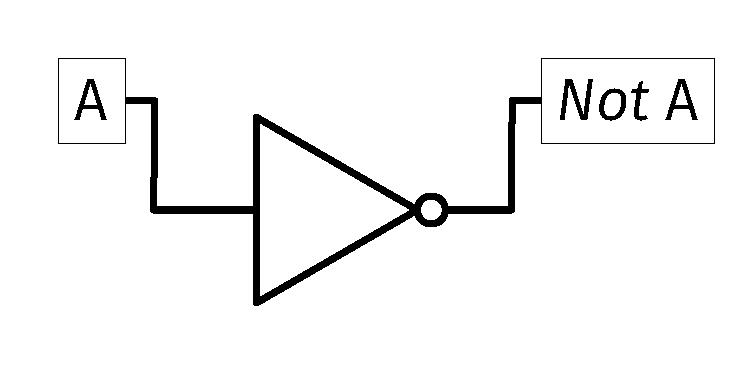
\includegraphics[width=0.5\textwidth]{figures/NOTOperation.pdf}
\caption{\label{fig:NOT} The inverter performs the complement operation at gate-level, $\overline{A} = NOT~A$.}
\end{figure}
\end{frame}

\begin{frame}{Boolean Algebra Basics}
\small
\textit{AND is multiplication, and OR is addition.  Refer to Chapter 2 DF.} \\ \vspace{0.1cm}
\textbf{Boolean or logical algebra} has these \textit{properties}:
\begin{enumerate}
\item \alert{Property of commutativity}
\begin{itemize}
\item \textbf{Addition version: $A + B = B + A$}
\item (\textit{an OR gate does not distinguish between inputs})
\item \textbf{Mutliplication version: $AB = BA$}
\item (\textit{an AND gate does not distinguish between inputs})
\end{itemize}
\item \alert{Property of Associativity}
\begin{itemize}
\item \textbf{Addition version: $(A+B)+C = A+(B+C)$}
\item \textit{OR gate order does not matter}.
\item \textbf{Mutliplication version: $(AB)C = A(BC)$}
\item \textit{AND gate order does not matter}.
\end{itemize}
\item \alert{Property of Distribution}
\begin{itemize}
\item $A(B+C) = AB+BC$ (\textit{gate input and gate order})
\end{itemize}
\end{enumerate}
\end{frame}

\begin{frame}{Boolean Algebra Basics}
\small
\begin{columns}[T]
\begin{column}{0.5\textwidth}
\textbf{Boolean or logical algebra} has these \textit{rules}:
\begin{enumerate}
\item $A+0 = A$
\item $A+1=1$
\item $A\cdot 0=0$
\item $A\cdot 1=A$
\item $A+A=A$
\item $A+\overline{A}=1$
\item $AA = A$
\item $A\overline{A}=0$
\item $\overline{\overline{A}} = A$
\end{enumerate}
\end{column}
\begin{column}{0.5\textwidth}
\textbf{Boolean or logical algebra} has these \textit{special rules}:
\begin{enumerate}
\item $A+AB = A$
\item $A+\overline{A}B=A+B$
\item $(A+B)(A+C) = A+BC$
\end{enumerate} \vspace{0.2cm}
\tiny
\textbf{Exercises:} \\ \hrulefill
\begin{itemize}
\item Prove special rule (1) with a truth table
\item Why is special rule (1) intuitive?
\item Prove special rule (2) with a truth table
\item Why is special rule (2) intuitive?
\item \textbf{Group board exercise:} Prove special rule (3) \textit{Hint: this requires rules 2, 4, and 7.  This is good practice at \textbf{gate simplification.}}
\end{itemize}
\end{column}
\end{columns}
\end{frame}

\begin{frame}{Boolean Algebra Basics}
\begin{columns}[T]
\begin{column}{0.5\textwidth}
De Morgan's Theorems \\ \hrulefill
\begin{itemize}
\small
\item \textbf{First theorem}: The complement of a product of literals is equal to the sum of the complements of the literals.
\item \textbf{Second theorem}: The complement of a sum of literals is equal to the product of the complements of the literals.
\end{itemize}
\end{column}
\begin{column}{0.5\textwidth}
\begin{itemize}
\item First theorem: $\overline{AB} = \overline{A}+\overline{B}$
\item Second theorem: $\overline{A+B} = \overline{A}\overline{B}$
\end{itemize} \hrulefill \\
For example: \\ 
$\overline{(AB+BC)} = \overline{AB}~\overline{BC} = (\overline{A}+\overline{B})(\overline{B}+\overline{C})$
\end{column}
\end{columns}
\end{frame}

\begin{frame}{Boolean Algebra Basics}
\small
\textbf{Group board exercise}: Show that
\begin{equation}
\begin{multlined}
\boxed{
\overline{(A+B)(B+C)}+\overline{(A+\overline{A}B)(B+\overline{B}A)}=\overline{A}+\overline{B}+\overline{C}} \label{eq:prob1}
\end{multlined}
\end{equation}
\begin{itemize}
\item \textit{Hint}: use De Morgan's two theorems
\item \textit{Hint}: use special rules
\item \textit{Hint}: consider the regular rules
\end{itemize}
\textbf{Group board exercise}: Create a circuit using logic gates that represents the left-hand side of Eq. \ref{eq:prob1}, and do the same for the right-hand side.  How many gates fewer are there in the right-hand solution?
\end{frame}

\begin{frame}{Boolean Algebra Basics}
\small
\textbf{Group board exercise}: Show that
\begin{equation}
\boxed{
\begin{multlined}
(AB+C(B+A))+\overline{(AB+C(B+A))}(AC+B(C+A)) \\ = AB+AC+BC \label{eq:prob2}
\end{multlined}}
\end{equation}
\begin{itemize}
\item \textit{Hint}: use special rules
\item \textit{Hint}: use De Morgan's two theorems
\end{itemize}
\textbf{Group board exercise}: Create a circuit using logic gates that represents the left-hand side of Eq. \ref{eq:prob2}, and do the same for the right-hand side.  How many gates fewer are there in the right-hand solution?
\end{frame}

\begin{frame}{Boolean Algebra Basics}
\begin{figure}
\centering
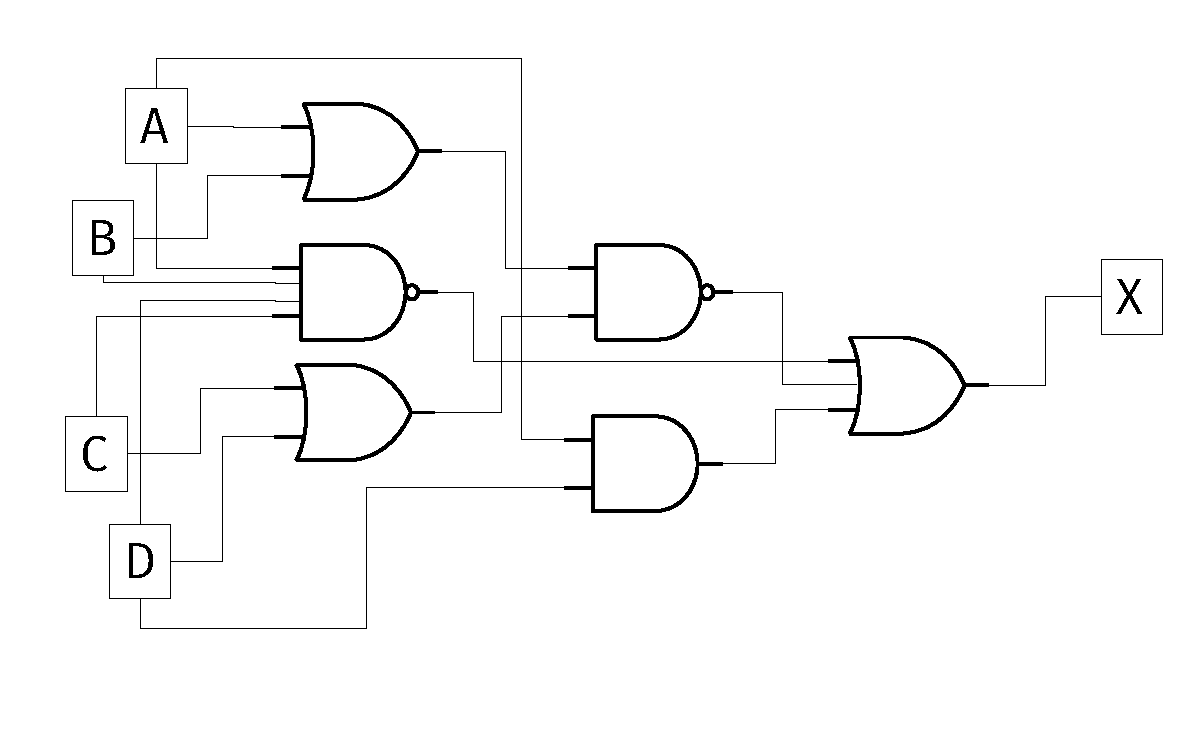
\includegraphics[width=0.8\textwidth]{figures/MultiGate1.pdf}
\caption{\label{fig:multi1} (1) Derive the logical algebraic expression for $X$.  (2) Proceed left to right.  (3) Simplify the result using simple rules. (4) Draw the equivalent circuit using gates.}
\end{figure}
\end{frame}

\begin{frame}{Boolean Algebra Basics}
\begin{figure}
\centering
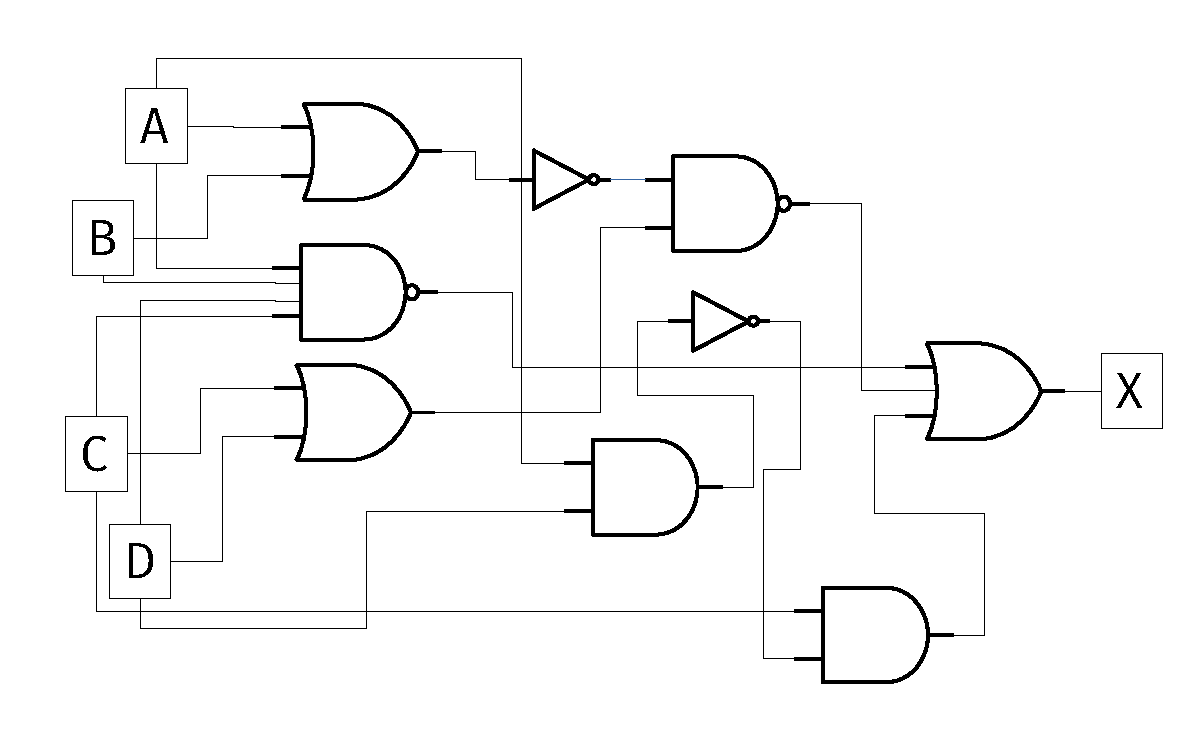
\includegraphics[width=0.8\textwidth]{figures/MultiGate2.pdf}
\caption{\label{fig:multi2} (1) Derive the logical algebraic expression for $X$.  (2) Proceed left to right.  (3) Simplify the result using simple rules. (4) Draw the equivalent circuit using gates.}
\end{figure}
\end{frame}

\begin{frame}{Boolean Algebra Basics}
\begin{figure}
\centering
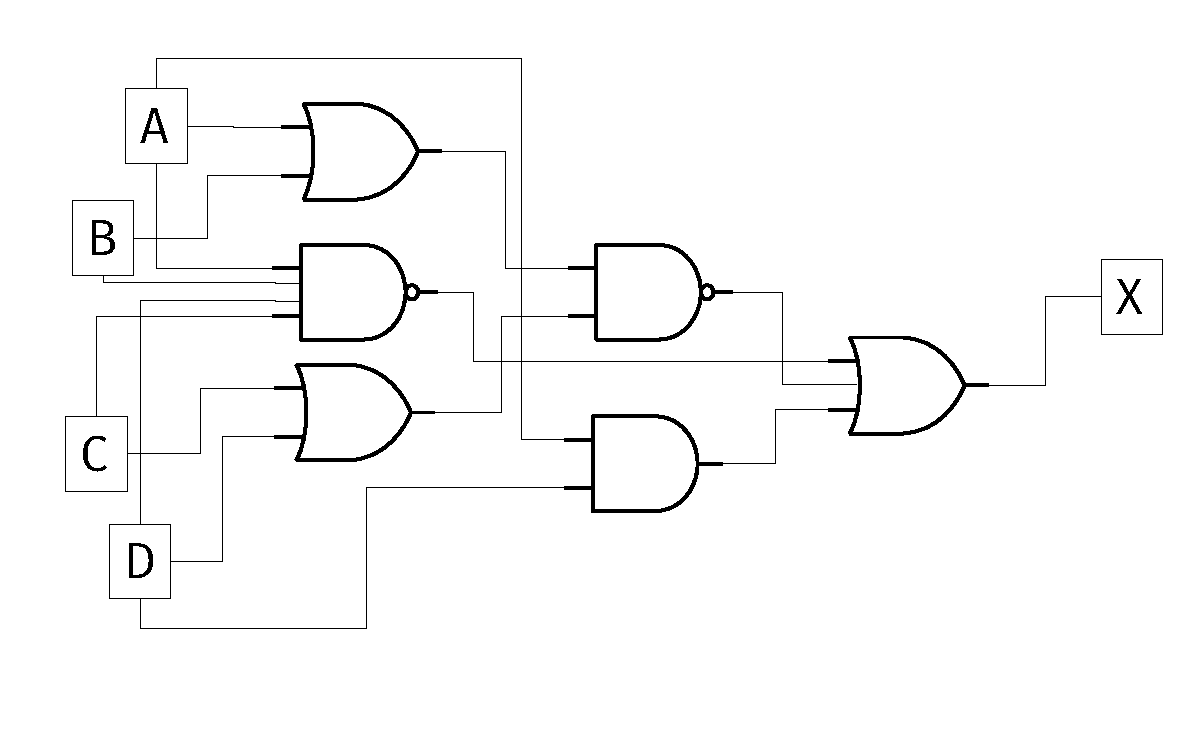
\includegraphics[width=0.8\textwidth]{figures/MultiGate1.pdf}
\caption{\label{fig:multi3} Construct the truth table.}
\end{figure}
\end{frame}

\begin{frame}{Boolean Algebra Basics}
\begin{figure}
\centering
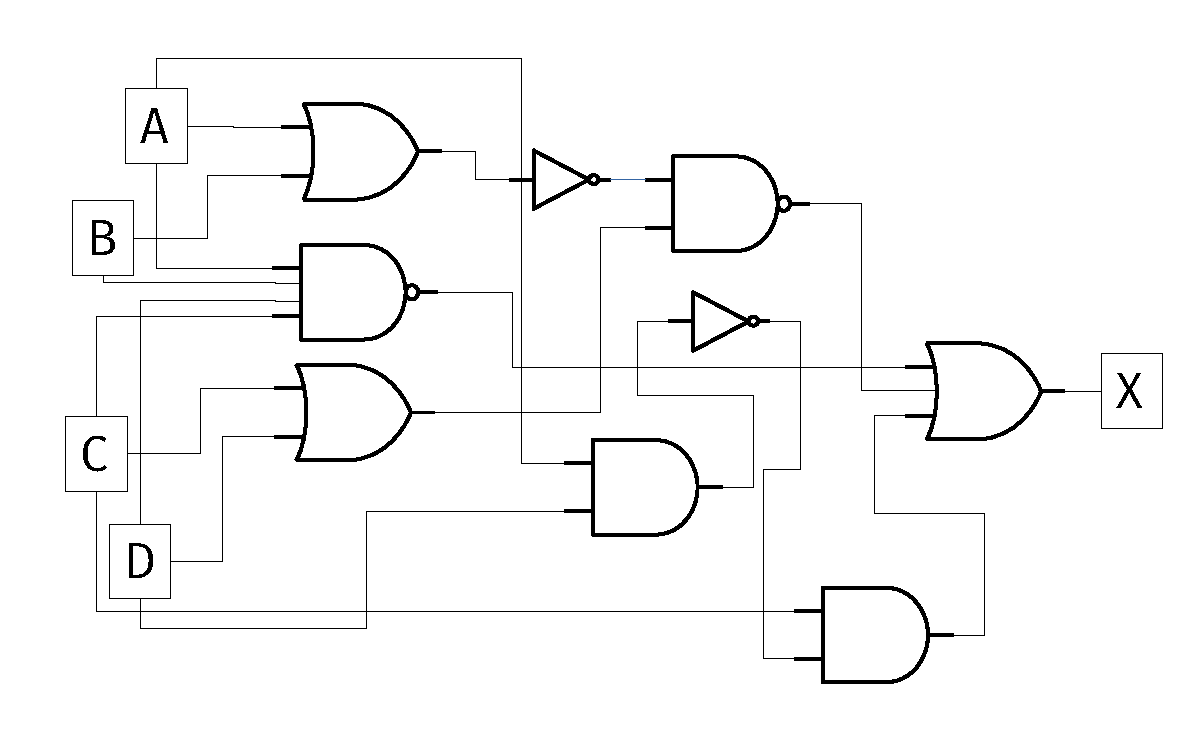
\includegraphics[width=0.8\textwidth]{figures/MultiGate2.pdf}
\caption{\label{fig:multi4} Construct the truth table.}
\end{figure}
\end{frame}

\section{SOP and POS Minimization}

\begin{frame}{SOP and POS Minimization}
Is there a standard way for performing these actions? \\ \hrulefill \\
\alert{SOP - \textit{Sum of products} form.} \\
\alert{POS} - \textit{Product of sums} form. \\ \hrulefill \\
\textbf{Rules for SOP form:}
\begin{enumerate}
\item All terms must be grouped by OR operations
\item No complements of literal groups, e.g. $\overline{ABD}$
\item Example: $A + \overline{B} + AB + ABCD$
\end{enumerate}
\end{frame}

\begin{frame}{SOP and POS Minimization}
\alert{SOP} - \textit{Sum of products} form. \\
\alert{S-SOP} - \textbf{Standard} \textit{Sum of products} form. \\ \hrulefill \\
\textbf{Rules for S-SOP form:}
\begin{enumerate}
\item All terms must be grouped by OR operations
\item No complements of literal groups, e.g. $\overline{ABD}$
\item Each term must \textit{span the domain} of literals
\item Example: $ABC + A\overline{B}C + AB\overline{C}$
\end{enumerate}
Notice that S-SOP is not necessarily the simplest form, but it has a different usage.
\end{frame}

\begin{frame}{SOP and POS Minimization}
\textbf{Build the truth table for this S-SOP expression:}
\begin{equation}
X = \overline{A}BCD+A\overline{B}CD
\end{equation}
\begin{enumerate}
\item How many input combinations are there?
\item How many input combinations result in $X = TRUE$?
\end{enumerate}
\end{frame}

\begin{frame}{SOP and POS Minimization}
\begin{equation}
X = \overline{A}BCD+A\overline{B}CD \label{eq:S-SOP}
\end{equation}
\tiny
\begin{table}
\begin{tabular}{c c c c c}
\textbf{A} & \textbf{B} & \textbf{C} & \textbf{D} & \textbf{X} \\
0 & 0 & 0 & 0 & 0 \\
0 & 0 & 0 & 1 & 0 \\
0 & 0 & 1 & 0 & 0 \\
0 & 0 & 1 & 1 & 0 \\
0 & 1 & 0 & 0 & 0 \\
0 & 1 & 0 & 1 & 0 \\
0 & 1 & 1 & 0 & 0 \\ \hline
\textbf{0} & \textbf{1} & \textbf{1} & \textbf{1} & \textbf{1} \\ \hline
1 & 0 & 0 & 0 & 0 \\
1 & 0 & 0 & 1 & 0 \\
1 & 0 & 1 & 0 & 0 \\ \hline
\textbf{1} & \textbf{0} & \textbf{1} & \textbf{1} & \textbf{1} \\ \hline
1 & 1 & 0 & 0 & 0 \\
1 & 1 & 0 & 1 & 0 \\
1 & 1 & 1 & 0 & 0 \\
1 & 1 & 1 & 1 & 0 \\
\end{tabular}
\caption{\label{tab:TT1} Truth table for Eq. \ref{eq:S-SOP}. S-SOP makes identifying TRUE final states trivial by identifying TRUE codes for individual terms.}
\end{table}
\end{frame}

\begin{frame}{SOP and POS Minimization}
\small
How do we convert to SOP and then S-SOP form?
\begin{enumerate}
\item SOP: expand terms using De Morgan's theorems and simple rules
\item S-SOP: use rule 6: $A+\overline{A} = 1$ to complete the domain of each OR term
\end{enumerate} \hrulefill \\
\textbf{Example:} The domain is $ABCD$
\begin{align}
X &= A\overline{B}+BC(A+D) \\
X &= A\overline{B}+ABC+BCD \\
X &= A\overline{B}(C+\overline{C})(D+\overline{D}) + ABC(D+\overline{D}) + (A+\overline{A})BCD \\
X &= A\overline{B}CD+A\overline{B}~\overline{C}~\overline{D} + ABCD+ABC\overline{D} + ABCD+\overline{A}BCD \label{eq:S-SOP2}
\end{align}
\textbf{(1) How many unique TRUE states exist for X? (2) Which input codes make X TRUE?}
\end{frame}

\begin{frame}{SOP and POS Minimization}
Is there a standard way for performing these actions? \\ \hrulefill \\
\alert{SOP} - \textit{Sum of products} form. \\
\alert{POS - \textit{Product of sums} form.} \\ \hrulefill \\
\textbf{Rules for POS form:}
\begin{enumerate}
\item All terms must be grouped by AND operations
\item No complements of literal sums, e.g. $\overline{A+D}$
\item Example: $(A+C)(A+\overline{B}+C)$
\end{enumerate}
\end{frame}

\begin{frame}{SOP and POS Minimization}
\alert{POS} - \textit{Product of sums} form. \\
\alert{S-POS - \textbf{Standard} \textit{Product of sums} form.} \\ \hrulefill \\
\textbf{Rules for S-POS form:}
\begin{enumerate}
\item All terms must be grouped by AND operations
\item No complements of literal sums, e.g. $\overline{A+D}$
\item Each term must \textit{span the domain} of literals
\item Example: $(A+B+C)(A+\overline{B}+C)$
\end{enumerate}
Notice that S-POS is not necessarily the simplest form, but it has a different usage.
\end{frame}

\begin{frame}{SOP and POS Minimization}
\textbf{Build the truth table for this S-POS expression:}
\begin{equation}
X = (A+B+C+D)(\overline{A}+B+C+D)(A+\overline{B}+C+D)(A+B+\overline{C}+D)
\end{equation}
\begin{enumerate}
\item How many input combinations are there?
\item How many input combinations result in $X = FALSE$?
\end{enumerate}
\end{frame}

\begin{frame}{SOP and POS Minimization}
\begin{equation}
X = (A+B+C+D)(\overline{A}+B+C+D)(A+\overline{B}+C+D)(A+B+\overline{C}+D) \label{eq:S-POS}
\end{equation}
\tiny
\begin{table}
\begin{tabular}{c c c c c}
\textbf{A} & \textbf{B} & \textbf{C} & \textbf{D} & \textbf{X} \\ \hline
\textbf{0} & \textbf{0} & \textbf{0} & \textbf{0} & \textbf{0} \\ \hline
0 & 0 & 0 & 1 & 1 \\ \hline
\textbf{0} & \textbf{0} & \textbf{1} & \textbf{0} & \textbf{0} \\ \hline
0 & 0 & 1 & 1 & 1 \\ \hline
\textbf{0} & \textbf{1} & \textbf{0} & \textbf{0} & \textbf{0} \\ \hline
0 & 1 & 0 & 1 & 1 \\
0 & 1 & 1 & 0 & 1 \\
0 & 1 & 1 & 1 & 1 \\ \hline
\textbf{1} & \textbf{0} & \textbf{0} & \textbf{0} & \textbf{0} \\ \hline
1 & 0 & 0 & 1 & 1 \\
1 & 0 & 1 & 0 & 1 \\
1 & 0 & 1 & 1 & 1 \\
1 & 1 & 0 & 0 & 1 \\
1 & 1 & 0 & 1 & 1 \\
1 & 1 & 1 & 0 & 1 \\
1 & 1 & 1 & 1 & 1 \\
\end{tabular}
\caption{\label{tab:TT2} Truth table for Eq. \ref{eq:S-POS}. S-POS makes identifying FALSE final states trivial by identifying FALSE codes for individual terms.}
\end{table}
\end{frame}

\begin{frame}{SOP and POS Minimization}
\small
How do we convert to POS and then S-POS form?
\begin{enumerate}
\item POS: Factor terms using De Morgan's theorems and simple rules
\item S-POS: Add a rule 8 pair to terms not spanning domain: $A\overline{A}$
\item Apply rule 12 to this term: $A+BC = (A+B)(A+C)$
\item (Looks like this: $A+B\overline{B} = (A+B)(A+\overline{B})$)
\end{enumerate} \hrulefill \\
\textbf{Example:} The domain is $ABCD$
\begin{align}
X &= (A\overline{B}+C+D)+(A+C) \\
X &= (A\overline{B}+C+D) + (A+C+B\overline{B}) \\
X &= K+(Q+B\overline{B}) \\
X &= K+(Q+B)(Q+\overline{B}) \\
... & ~ (continued)
\end{align}
\end{frame}

\begin{frame}{SOP and POS Minimization}
\small
How do we convert to POS and then S-POS form?
\begin{enumerate}
\item POS: Factor terms using De Morgan's theorems and simple rules
\item S-POS: Add a rule 8 pair to terms not spanning domain: $A\overline{A}$
\item Apply rule 12 to this term: $A+BC = (A+B)(A+C)$
\item (Looks like this: $A+B\overline{B} = (A+B)(A+\overline{B})$)
\end{enumerate} \hrulefill \\
\textbf{Example:} The domain is $ABCD$
\begin{align}
X &= K+(Q+B)(Q+\overline{B}) \\
X &= (K+Q+B)(K+Q+\overline{B}) \\
X &= (A+B+C+D)(A+\overline{B}+C+D) \label{eq:S-POS2}
\end{align}
\textbf{(1) How many unique FALSE states exist for X? (2) Which input codes make X FALSE?}
\end{frame}

\begin{frame}{SOP and POS Minimization}
\textbf{Conversions between S-SOP and S-POS} \\ \hrulefill \\
\begin{columns}[T]
\small
\begin{column}{0.5\textwidth}
\centering
SOP to POS
\begin{enumerate}
\item Determine domain size
\item Identify TRUE codes
\item \alert{Remaining codes are the FALSE codes for POS}
\item Write sum terms corresponding to the FALSE codes
\item Multiply all sum terms
\end{enumerate}
\end{column}
\begin{column}{0.5\textwidth}
\centering
POS to SOP
\begin{enumerate}
\item Determine domain size
\item Identify FALSE codes
\item \alert{Remaining codes are the TRUE codes for SOP}
\item Write product terms corresponding to the TRUE codes
\item Add all product terms
\end{enumerate}
\end{column}
\end{columns}
\textbf{The bottom line: a code cannot give both a TRUE and FALSE answer.}
\end{frame}

\begin{frame}{SOP and POS Minimization}
\textbf{Exercise:} Convert the following from SOP to POS:
\begin{equation}
\overline{A}~\overline{B}~\overline{C}+\overline{A}B\overline{C}+\overline{A}BC+A\overline{B}C+ABC = X
\end{equation}
\end{frame}

\begin{frame}{SOP and POS Minimization}
\textbf{Exercise:} Convert the following from SOP to POS:
\begin{equation}
\overline{A}~\overline{B}~\overline{C}+\overline{A}B\overline{C}+\overline{A}BC+A\overline{B}C+ABC = X
\end{equation}
\begin{itemize}
\item TRUE codes: 000, 010, 011, 101, 111
\item FALSE codes for POS: 001, 100, 110
\item First false code sum-term: $(A+B+\overline{C})$, ...
\end{itemize}
\end{frame}

\begin{frame}{SOP and POS Minimization}
\textit{Using similar strategies, SOP and POS expressions can be derived from a truth table (TT).}  The converse is simpler: convert to S-SOP or S-POS and fill in the table.
\begin{columns}[T]
\small
\begin{column}{0.5\textwidth}
\centering
TT to S-SOP
\begin{enumerate}
\item Locate TRUE final states in TT
\item Write the input codes as product terms, replacing 1's with literals and 0's with complements
\item Sum the product terms
\end{enumerate}
\end{column}
\begin{column}{0.5\textwidth}
\centering
TT to S-POS
\begin{enumerate}
\item Locate FALSE final states in TT
\item Write the input codes as sum terms, replacing 1's with complement and 0's with literals.
\item Multiply the sum terms
\end{enumerate}
\end{column}
\end{columns}
\end{frame}

\begin{frame}{SOP and POS Minimization}
\textbf{Where it gets interesting:} \\ \vspace{0.5cm}
Design requirements $\rightarrow$ TT $\rightarrow$ S-SOP or S-POS $\rightarrow$ Simplification via De Morgan's/simple and special rules $\rightarrow$ digital circuit design \\ \vspace{0.5cm}
\begin{columns}[T]
\small
\begin{column}{0.5\textwidth}
``Ya know Bob..I think we need it to do this new action...'' $\rightarrow$
\end{column}
\begin{column}{0.5\textwidth}
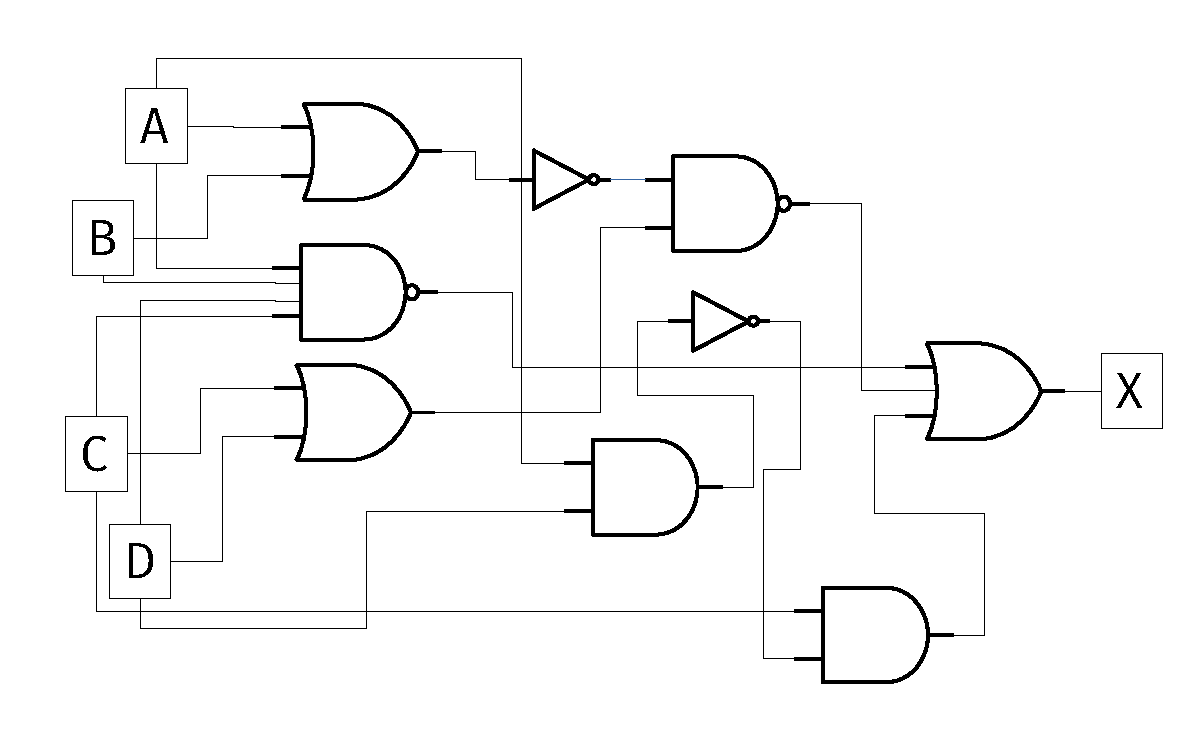
\includegraphics[width=0.9\textwidth]{figures/MultiGate2.pdf}
\end{column}
\end{columns}
\textbf{Before going there, we will discuss Karnaugh maps next time.}
\end{frame}

\section{Conclusion}

\begin{frame}{Unit 2 Conclusion - Theoretical Logic Gates, and Operations}
\begin{enumerate}
\item Logic Gates
\begin{itemize}
\item Circuit diagram
\item Truth table
\item Timing diagram
\item Boolean logic
\end{itemize}
\item \alert{Boolean algebra I} ... Expressions, rules, simplification
\item \alert{Boolean algebra II} ... SOP, POS, Karnaugh Maps
\end{enumerate}
\end{frame}

\end{document}
